\documentclass[twoside]{book}

% Packages required by doxygen
\usepackage{fixltx2e}
\usepackage{calc}
\usepackage{doxygen}
\usepackage[export]{adjustbox} % also loads graphicx
\usepackage{graphicx}
\usepackage[utf8]{inputenc}
\usepackage{makeidx}
\usepackage{multicol}
\usepackage{multirow}
\PassOptionsToPackage{warn}{textcomp}
\usepackage{textcomp}
\usepackage[nointegrals]{wasysym}
\usepackage[table]{xcolor}

% Font selection
\usepackage[T1]{fontenc}
\usepackage[scaled=.90]{helvet}
\usepackage{courier}
\usepackage{amssymb}
\usepackage{sectsty}
\renewcommand{\familydefault}{\sfdefault}
\allsectionsfont{%
  \fontseries{bc}\selectfont%
  \color{darkgray}%
}
\renewcommand{\DoxyLabelFont}{%
  \fontseries{bc}\selectfont%
  \color{darkgray}%
}
\newcommand{\+}{\discretionary{\mbox{\scriptsize$\hookleftarrow$}}{}{}}

% Page & text layout
\usepackage{geometry}
\geometry{%
  a4paper,%
  top=2.5cm,%
  bottom=2.5cm,%
  left=2.5cm,%
  right=2.5cm%
}
\tolerance=750
\hfuzz=15pt
\hbadness=750
\setlength{\emergencystretch}{15pt}
\setlength{\parindent}{0cm}
\setlength{\parskip}{3ex plus 2ex minus 2ex}
\makeatletter
\renewcommand{\paragraph}{%
  \@startsection{paragraph}{4}{0ex}{-1.0ex}{1.0ex}{%
    \normalfont\normalsize\bfseries\SS@parafont%
  }%
}
\renewcommand{\subparagraph}{%
  \@startsection{subparagraph}{5}{0ex}{-1.0ex}{1.0ex}{%
    \normalfont\normalsize\bfseries\SS@subparafont%
  }%
}
\makeatother

% Headers & footers
\usepackage{fancyhdr}
\pagestyle{fancyplain}
\fancyhead[LE]{\fancyplain{}{\bfseries\thepage}}
\fancyhead[CE]{\fancyplain{}{}}
\fancyhead[RE]{\fancyplain{}{\bfseries\leftmark}}
\fancyhead[LO]{\fancyplain{}{\bfseries\rightmark}}
\fancyhead[CO]{\fancyplain{}{}}
\fancyhead[RO]{\fancyplain{}{\bfseries\thepage}}
\fancyfoot[LE]{\fancyplain{}{}}
\fancyfoot[CE]{\fancyplain{}{}}
\fancyfoot[RE]{\fancyplain{}{\bfseries\scriptsize Generated by Doxygen }}
\fancyfoot[LO]{\fancyplain{}{\bfseries\scriptsize Generated by Doxygen }}
\fancyfoot[CO]{\fancyplain{}{}}
\fancyfoot[RO]{\fancyplain{}{}}
\renewcommand{\footrulewidth}{0.4pt}
\renewcommand{\chaptermark}[1]{%
  \markboth{#1}{}%
}
\renewcommand{\sectionmark}[1]{%
  \markright{\thesection\ #1}%
}

% Indices & bibliography
\usepackage{natbib}
\usepackage[titles]{tocloft}
\setcounter{tocdepth}{3}
\setcounter{secnumdepth}{5}
\makeindex

% Hyperlinks (required, but should be loaded last)
\usepackage{ifpdf}
\ifpdf
  \usepackage[pdftex,pagebackref=true]{hyperref}
\else
  \usepackage[ps2pdf,pagebackref=true]{hyperref}
\fi
\hypersetup{%
  colorlinks=true,%
  linkcolor=blue,%
  citecolor=blue,%
  unicode%
}

% Custom commands
\newcommand{\clearemptydoublepage}{%
  \newpage{\pagestyle{empty}\cleardoublepage}%
}

\usepackage{caption}
\captionsetup{labelsep=space,justification=centering,font={bf},singlelinecheck=off,skip=4pt,position=top}

%===== C O N T E N T S =====

\begin{document}

% Titlepage & ToC
\hypersetup{pageanchor=false,
             bookmarksnumbered=true,
             pdfencoding=unicode
            }
\pagenumbering{alph}
\begin{titlepage}
\vspace*{7cm}
\begin{center}%
{\Large My Project }\\
\vspace*{1cm}
{\large Generated by Doxygen 1.8.13}\\
\end{center}
\end{titlepage}
\clearemptydoublepage
\pagenumbering{roman}
\tableofcontents
\clearemptydoublepage
\pagenumbering{arabic}
\hypersetup{pageanchor=true}

%--- Begin generated contents ---
\chapter{Class Index}
\section{Class List}
Here are the classes, structs, unions and interfaces with brief descriptions\+:\begin{DoxyCompactList}
\item\contentsline{section}{\hyperlink{structcrecmap_1_1map__region}{crecmap\+::map\+\_\+region} }{\pageref{structcrecmap_1_1map__region}}{}
\item\contentsline{section}{\hyperlink{structcrecmap_1_1mbb__node}{crecmap\+::mbb\+\_\+node} }{\pageref{structcrecmap_1_1mbb__node}}{}
\item\contentsline{section}{\hyperlink{structcrecmap_1_1mbb__set}{crecmap\+::mbb\+\_\+set} }{\pageref{structcrecmap_1_1mbb__set}}{}
\item\contentsline{section}{\hyperlink{classcrecmap_1_1RecMap}{crecmap\+::\+Rec\+Map} }{\pageref{classcrecmap_1_1RecMap}}{}
\end{DoxyCompactList}

\chapter{Class Documentation}
\hypertarget{structcrecmap_1_1map__region}{}\section{crecmap\+:\+:map\+\_\+region Struct Reference}
\label{structcrecmap_1_1map__region}\index{crecmap\+::map\+\_\+region@{crecmap\+::map\+\_\+region}}


Collaboration diagram for crecmap\+:\+:map\+\_\+region\+:\nopagebreak
\begin{figure}[H]
\begin{center}
\leavevmode
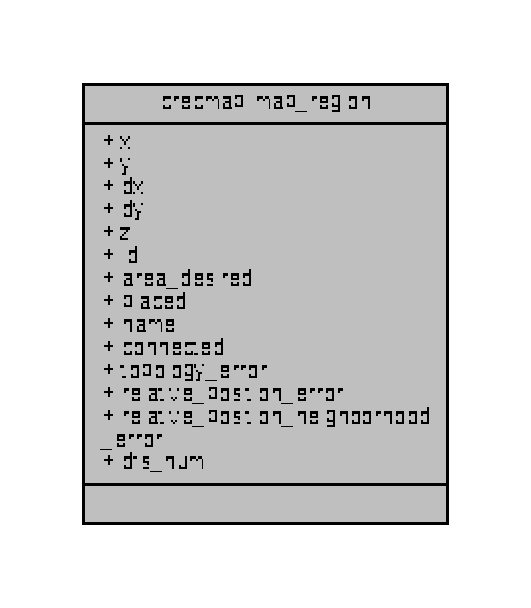
\includegraphics[width=255pt]{structcrecmap_1_1map__region__coll__graph}
\end{center}
\end{figure}
\subsection*{Public Attributes}
\begin{DoxyCompactItemize}
\item 
\mbox{\Hypertarget{structcrecmap_1_1map__region_af97de6d9252476764e052567b4db4245}\label{structcrecmap_1_1map__region_af97de6d9252476764e052567b4db4245}} 
double {\bfseries x}
\item 
\mbox{\Hypertarget{structcrecmap_1_1map__region_ab1c494cbbd70260988a36ea97861fdaa}\label{structcrecmap_1_1map__region_ab1c494cbbd70260988a36ea97861fdaa}} 
double {\bfseries y}
\item 
\mbox{\Hypertarget{structcrecmap_1_1map__region_a18f763b6bae24cc9eb05c52900b7b6db}\label{structcrecmap_1_1map__region_a18f763b6bae24cc9eb05c52900b7b6db}} 
double {\bfseries dx}
\item 
\mbox{\Hypertarget{structcrecmap_1_1map__region_accd40f846b5f71a946faa5af3766c5ca}\label{structcrecmap_1_1map__region_accd40f846b5f71a946faa5af3766c5ca}} 
double {\bfseries dy}
\item 
\mbox{\Hypertarget{structcrecmap_1_1map__region_a3c8ca629979ccd7b2a281a2e84b37b8d}\label{structcrecmap_1_1map__region_a3c8ca629979ccd7b2a281a2e84b37b8d}} 
double {\bfseries z}
\item 
\mbox{\Hypertarget{structcrecmap_1_1map__region_a4695e166e93d4929524699e337183b0f}\label{structcrecmap_1_1map__region_a4695e166e93d4929524699e337183b0f}} 
int {\bfseries id}
\item 
\mbox{\Hypertarget{structcrecmap_1_1map__region_a0871482039e61a3006b2646a33b028e4}\label{structcrecmap_1_1map__region_a0871482039e61a3006b2646a33b028e4}} 
double {\bfseries area\+\_\+desired}
\item 
\mbox{\Hypertarget{structcrecmap_1_1map__region_afc41f4e791380ef057a5ca94d94be64d}\label{structcrecmap_1_1map__region_afc41f4e791380ef057a5ca94d94be64d}} 
int {\bfseries placed}
\item 
\mbox{\Hypertarget{structcrecmap_1_1map__region_aab1330fcd69e4a86a748eee70fdd51c2}\label{structcrecmap_1_1map__region_aab1330fcd69e4a86a748eee70fdd51c2}} 
std\+::string {\bfseries name}
\item 
\mbox{\Hypertarget{structcrecmap_1_1map__region_aa1917d7aa0720c507f260374f11516fe}\label{structcrecmap_1_1map__region_aa1917d7aa0720c507f260374f11516fe}} 
std\+::vector$<$ int $>$ {\bfseries connected}
\item 
\mbox{\Hypertarget{structcrecmap_1_1map__region_a9023cf4658ce2f21290b62c2e2ee9401}\label{structcrecmap_1_1map__region_a9023cf4658ce2f21290b62c2e2ee9401}} 
double {\bfseries topology\+\_\+error}
\item 
\mbox{\Hypertarget{structcrecmap_1_1map__region_a83e9ccaa7694718d4dfa6c8c2f2593ef}\label{structcrecmap_1_1map__region_a83e9ccaa7694718d4dfa6c8c2f2593ef}} 
double {\bfseries relative\+\_\+position\+\_\+error}
\item 
\mbox{\Hypertarget{structcrecmap_1_1map__region_aed781775ed47c4af24b3c2a76f232f46}\label{structcrecmap_1_1map__region_aed781775ed47c4af24b3c2a76f232f46}} 
double {\bfseries relative\+\_\+position\+\_\+neighborhood\+\_\+error}
\item 
\mbox{\Hypertarget{structcrecmap_1_1map__region_a80f4d9d2679093cc81fac7a0bbc8c2b2}\label{structcrecmap_1_1map__region_a80f4d9d2679093cc81fac7a0bbc8c2b2}} 
int {\bfseries dfs\+\_\+num}
\end{DoxyCompactItemize}


The documentation for this struct was generated from the following file\+:\begin{DoxyCompactItemize}
\item 
recmap.\+h\end{DoxyCompactItemize}

\hypertarget{structcrecmap_1_1mbb__node}{\section{crecmap\+:\+:mbb\+\_\+node Struct Reference}
\label{structcrecmap_1_1mbb__node}\index{crecmap\+::mbb\+\_\+node@{crecmap\+::mbb\+\_\+node}}
}
\subsection*{Public Member Functions}
\begin{DoxyCompactItemize}
\item 
\hypertarget{structcrecmap_1_1mbb__node_a74749cee5a8b35777ec9bb7d967b2050}{{\bfseries mbb\+\_\+node} (const double \&str\+Key=0, const int \&int\+Id=0)}\label{structcrecmap_1_1mbb__node_a74749cee5a8b35777ec9bb7d967b2050}

\item 
\hypertarget{structcrecmap_1_1mbb__node_a9be94f8ce6bef4b6d17f94a309622d20}{bool {\bfseries operator$<$} (const \hyperlink{structcrecmap_1_1mbb__node}{mbb\+\_\+node} \&rhs) const }\label{structcrecmap_1_1mbb__node_a9be94f8ce6bef4b6d17f94a309622d20}

\end{DoxyCompactItemize}
\subsection*{Public Attributes}
\begin{DoxyCompactItemize}
\item 
\hypertarget{structcrecmap_1_1mbb__node_a17fd42b192941d75a018fcd8221535f9}{double {\bfseries key}}\label{structcrecmap_1_1mbb__node_a17fd42b192941d75a018fcd8221535f9}

\item 
\hypertarget{structcrecmap_1_1mbb__node_a3fa0677553f7e9971593cd65a295d78c}{int {\bfseries id}}\label{structcrecmap_1_1mbb__node_a3fa0677553f7e9971593cd65a295d78c}

\end{DoxyCompactItemize}


The documentation for this struct was generated from the following file\+:\begin{DoxyCompactItemize}
\item 
recmap.\+h\end{DoxyCompactItemize}

\hypertarget{structcrecmap_1_1mbb__set}{\section{crecmap\+:\+:mbb\+\_\+set Struct Reference}
\label{structcrecmap_1_1mbb__set}\index{crecmap\+::mbb\+\_\+set@{crecmap\+::mbb\+\_\+set}}
}
\subsection*{Public Attributes}
\begin{DoxyCompactItemize}
\item 
\hypertarget{structcrecmap_1_1mbb__set_a1307ff6aec408999c6f348bb42efa150}{double {\bfseries max\+\_\+dx}}\label{structcrecmap_1_1mbb__set_a1307ff6aec408999c6f348bb42efa150}

\item 
\hypertarget{structcrecmap_1_1mbb__set_a501f690ba4cbd602aec52c72c8abae05}{double {\bfseries max\+\_\+dy}}\label{structcrecmap_1_1mbb__set_a501f690ba4cbd602aec52c72c8abae05}

\item 
\hypertarget{structcrecmap_1_1mbb__set_a6dcb7bc9df15fd92ec6974cc876227de}{std\+::multiset$<$ \hyperlink{structcrecmap_1_1mbb__node}{mbb\+\_\+node} $>$ {\bfseries x}}\label{structcrecmap_1_1mbb__set_a6dcb7bc9df15fd92ec6974cc876227de}

\item 
\hypertarget{structcrecmap_1_1mbb__set_a63688e8e02c3a13bf971ea06bd3b084c}{std\+::multiset$<$ \hyperlink{structcrecmap_1_1mbb__node}{mbb\+\_\+node} $>$ {\bfseries y}}\label{structcrecmap_1_1mbb__set_a63688e8e02c3a13bf971ea06bd3b084c}

\end{DoxyCompactItemize}


The documentation for this struct was generated from the following file\+:\begin{DoxyCompactItemize}
\item 
recmap.\+h\end{DoxyCompactItemize}

\hypertarget{classcrecmap_1_1RecMap}{\section{crecmap\+:\+:Rec\+Map Class Reference}
\label{classcrecmap_1_1RecMap}\index{crecmap\+::\+Rec\+Map@{crecmap\+::\+Rec\+Map}}
}
\subsection*{Public Member Functions}
\begin{DoxyCompactItemize}
\item 
\hypertarget{classcrecmap_1_1RecMap_ad034322b3373816bfa8ea9e6c436d00d}{void {\bfseries push} (double x, double y, double dx, double dy, double z, std\+::string name)}\label{classcrecmap_1_1RecMap_ad034322b3373816bfa8ea9e6c436d00d}

\item 
\hypertarget{classcrecmap_1_1RecMap_a278f40f1df14d64df4c4a9cd5595da3b}{std\+::string {\bfseries warnings\+\_\+pop} ()}\label{classcrecmap_1_1RecMap_a278f40f1df14d64df4c4a9cd5595da3b}

\item 
\hypertarget{classcrecmap_1_1RecMap_a404641cf7fcf47dc32e101a823f6edb4}{bool {\bfseries warnings\+\_\+empty} ()}\label{classcrecmap_1_1RecMap_a404641cf7fcf47dc32e101a823f6edb4}

\item 
\hypertarget{classcrecmap_1_1RecMap_a77f39e195bb75242aac9bccd910b1307}{int {\bfseries get\+\_\+size} ()}\label{classcrecmap_1_1RecMap_a77f39e195bb75242aac9bccd910b1307}

\item 
\hypertarget{classcrecmap_1_1RecMap_a870136e4477ed8644ddc4a844f0b89f9}{int {\bfseries get\+\_\+intersect\+\_\+count} ()}\label{classcrecmap_1_1RecMap_a870136e4477ed8644ddc4a844f0b89f9}

\item 
\hypertarget{classcrecmap_1_1RecMap_a51c4a66b8b847749af400606b63940e9}{\hyperlink{structcrecmap_1_1map__region}{map\+\_\+region} \& {\bfseries get\+\_\+map\+\_\+region} (int i)}\label{classcrecmap_1_1RecMap_a51c4a66b8b847749af400606b63940e9}

\item 
\hypertarget{classcrecmap_1_1RecMap_a7284e0b346080f52476497c26ec61fd2}{void {\bfseries Compute\+Pseudo\+Dual} (recmapvector \&M)}\label{classcrecmap_1_1RecMap_a7284e0b346080f52476497c26ec61fd2}

\item 
\hypertarget{classcrecmap_1_1RecMap_ac738bcd3b60e52e29e6855fdea17b230}{void {\bfseries Compute\+Desired\+Area} (recmapvector \&M, recmapvector \&C)}\label{classcrecmap_1_1RecMap_ac738bcd3b60e52e29e6855fdea17b230}

\item 
\hypertarget{classcrecmap_1_1RecMap_a59c91bbd4b9d9c5057b082099f1bf89b}{int {\bfseries Compute\+Core\+Region} (recmapvector \&M, recmapvector \&C)}\label{classcrecmap_1_1RecMap_a59c91bbd4b9d9c5057b082099f1bf89b}

\item 
\hypertarget{classcrecmap_1_1RecMap_a18e096d369e0f4e4b2862af74367463d}{bool {\bfseries map\+\_\+region\+\_\+intersect} (const recmapvector \&C, const \hyperlink{structcrecmap_1_1map__region}{map\+\_\+region} \&a)}\label{classcrecmap_1_1RecMap_a18e096d369e0f4e4b2862af74367463d}

\item 
\hypertarget{classcrecmap_1_1RecMap_af5a5ca00e627d3f893734fb92eac2372}{bool {\bfseries map\+\_\+region\+\_\+intersect\+\_\+set} (recmapvector \&C, const \hyperlink{structcrecmap_1_1mbb__set}{mbb\+\_\+set} \&S, const \hyperlink{structcrecmap_1_1map__region}{map\+\_\+region} \&a)}\label{classcrecmap_1_1RecMap_af5a5ca00e627d3f893734fb92eac2372}

\item 
\hypertarget{classcrecmap_1_1RecMap_a9e8e3f05f71a8442fa7b259894f440e7}{bool {\bfseries Place\+Rectangle} (recmapvector \&M, recmapvector \&C, int region\+\_\+id)}\label{classcrecmap_1_1RecMap_a9e8e3f05f71a8442fa7b259894f440e7}

\item 
\hypertarget{classcrecmap_1_1RecMap_ac5e3a03d15aea4cd9ec532157b9b8268}{void {\bfseries Draw\+Cartogram} (recmapvector \&M, recmapvector \&C, int core\+\_\+region\+\_\+id)}\label{classcrecmap_1_1RecMap_ac5e3a03d15aea4cd9ec532157b9b8268}

\item 
\hypertarget{classcrecmap_1_1RecMap_a60be5dd2b1a501a9ef26724fae5d72ba}{void {\bfseries Compute\+Error} (const recmapvector \&M, recmapvector \&C)}\label{classcrecmap_1_1RecMap_a60be5dd2b1a501a9ef26724fae5d72ba}

\item 
\hypertarget{classcrecmap_1_1RecMap_a53f4cdc1bf45edbb3cf74bfa883d61ed}{void {\bfseries run} ()}\label{classcrecmap_1_1RecMap_a53f4cdc1bf45edbb3cf74bfa883d61ed}

\end{DoxyCompactItemize}


The documentation for this class was generated from the following file\+:\begin{DoxyCompactItemize}
\item 
recmap.\+h\end{DoxyCompactItemize}

%--- End generated contents ---

% Index
\backmatter
\newpage
\phantomsection
\clearemptydoublepage
\addcontentsline{toc}{chapter}{Index}
\printindex

\end{document}
